\documentclass[fleqn]{article}
\usepackage[spanish,es-noshorthands]{babel}
\usepackage[utf8]{inputenc} 
\usepackage[papersize={6.5in,8.5in},left=1cm, right=1cm, top=1.5cm, bottom=1.7cm]{geometry}
\usepackage{mathexam}
\usepackage{amsmath}
\usepackage{graphicx}
\usepackage{tikz,pgf}
\usepackage{tikz-3dplot}

\ExamClass{
\includegraphics[height=16pt]{Images/logo-sed.png} Matemáticas $9^{\circ}$}
\ExamName{`Nivelación áreas y volúmenes'}
\ExamHead{
\includegraphics[height=16pt]{Images/logo-colegio.png} IEDAB}
\newcommand{\LineaNombre}{%
\par
\vspace{\baselineskip}
Nombre:\hrulefill \; Curso: \underline{\hspace*{48pt}} \; Fecha: \underline{\hspace*{2.5cm}} \relax
\par}
\let\ds\displaystyle

\begin{document}
\ExamInstrBox{
Respuesta sin justificar mediante procedimiento no será tenida en cuenta en la calificación. Escriba sus respuestas en el espacio indicado. Tiene 45 minutos para contestar esta prueba.}
\LineaNombre
\begin{enumerate}
\item Para una tarea de artes Pedro sacó una fotocopia ampliada de la figura 1 y obtuvo la figura 2. Las figuras se muestran en la siguiente cuadrícula
\begin{center}
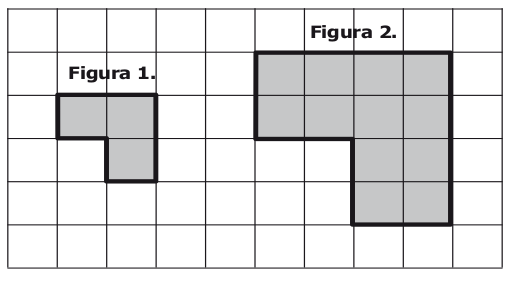
\includegraphics[scale=.5]{Images/areas.png} 
\end{center}
Es correcto afirmar que el área de la figura 2 es
\begin{enumerate}
\item tres veces el área de la figura 1
\item cuatro veces el área de la figura 1
\item igual al área de la figura 1
\item dos veces el área de la figura 1
\end{enumerate}

\begin{minipage}{.45\textwidth}
\tdplotsetmaincoords{70}{0}
\begin{tikzpicture}[tdplot_main_coords]
\def\RI{2}
\def\RII{2}

\draw[thick] (\RI,0)
  \foreach \x in {0,300,240,180} { --  (\x:\RI) node at (\x:\RI) (R1-\x) {} };
\draw[dashed,thick] (R1-0.center)
  \foreach \x in {60,120,180} { --  (\x:\RI) node at (\x:\RI) (R1-\x) {} };
\path[fill=gray!30] (\RI,0)
  \foreach \x in {0,60,120,180,240,300} { --  (\x:\RI)};

\begin{scope}[yshift=2cm]
\draw[thick,fill=gray!30,opacity=0.2] (\RII,0)
  \foreach \x in {0,60,120,180,240,300,360}
    { --  (\x:\RII) node at (\x:\RII) (R2-\x) {}};
\end{scope}

\foreach \x in {0,180,240,300} { \draw (R1-\x.center)--(R2-\x.center); };
\foreach \x in {60,120} { \draw[dashed] (R1-\x.center)--(R2-\x.center); };
\end{tikzpicture}
\end{minipage}
\begin{minipage}{.45\textwidth}
\item En la figura se muestra un prisma hexagonal. \textbf{NO} es correcto afirmar que el prisma tiene:
\begin{enumerate}
\item caras hexagonales.
\item 18 aristas.
\item 6 caras rectangulares.
\item 10 vértices.
\end{enumerate}
\end{minipage}

\begin{minipage}{.5\textwidth}
 \item Un carpintero construye un mueble que tiene cajones como el que aparece en la siguiente figura:
\begin{enumerate}
\item  ¿Cuál es la capacidad (volumen) en cm$^{3}$ de uno de los cajones del mueble?
\item ¿Cuánta maderá (en $cm^{2}$) necesitará para construir un cajón? (Recuerde que no tiene tapa superior)
\end{enumerate}
\end{minipage}
\begin{minipage}{.45\textwidth}
 \begin{center}
 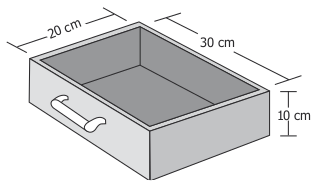
\includegraphics[scale=.6]{Images/Pantallazo-2.png} 
 \end{center}
\end{minipage}
\noanswer
\begin{minipage}{.35\textwidth}
\begin{tikzpicture}[scale=.5]
\fill[top color=gray!50!black,bottom color=gray!10,middle color=gray,shading=axis,opacity=0.25] (0,0) circle (2cm and 0.5cm);
\fill[left color=gray!50!black,right color=gray!50!black,middle color=gray!50,shading=axis,opacity=0.25] (2,0) -- (2,6) arc (360:180:2cm and 0.5cm) -- (-2,0) arc (180:360:2cm and 0.5cm);
\fill[top color=gray!90!,bottom color=gray!2,middle color=gray!30,shading=axis,opacity=0.25] (0,6) circle (2cm and 0.5cm);
\draw (-2,6) -- (-2,0) arc (180:360:2cm and 0.5cm) -- (2,6) ++ (-2,0) circle (2cm and 0.5cm);
\draw[densely dashed] (-2,0) arc (180:0:2cm and 0.5cm);
\draw[|-] (2.3,0) -- (2.3,2.7);
\node[right] (h) at (2,3) {$h$};
\draw[-|] (2.3,3.3) -- (2.3,6);
\draw (-2,6) --node[above]{$r$} (0,6);
\end{tikzpicture}
\end{minipage}
\begin{minipage}{.6\textwidth}
\item Calcule la superficie y el volumen del cilindo cuyo radio $r$ mide 3 cm y cuya altura $h$ mide 8 cm
\end{minipage}\noanswer
\begin{minipage}{.5\textwidth}
\item A un cilindro de 6 cm de altura y 6 cm de radio de la base, se le ha quitado un cono como muestra la figura. Halla el volumen de la pieza que resulta. (\emph{Recuerde que el volumen de un cono recto es la tercera parte del volumen de un cilindro recto})
\end{minipage}
\begin{minipage}{.45\textwidth}
\begin{tikzpicture}
\fill[top color=gray!50!black,bottom color=gray!10,middle color=gray,shading=axis,opacity=0.25] (0,0) circle (2cm and 0.5cm);
\fill[left color=gray!50!black,right color=gray!50!black,middle color=gray!50,shading=axis,opacity=0.25] (2,0) -- (0,-2) -- (-2,0) arc (180:360:2cm and 0.5cm);
\draw (-2,0) arc (180:360:2cm and 0.5cm) -- (0,-2) -- cycle;
\draw[densely dashed] (-2,0) arc (180:0:2cm and 0.5cm);
\draw (-2,0)--(-2,-2) arc [start angle=180,end angle=360,x radius=2,y radius=.5] --node[right]{$h$}(2,0);
\draw[dashed] (-2,-2) arc (180:0):2cm and 0.5cm);
\draw (0,-2) --node[below]{$r$} (2,-2);
\end{tikzpicture}
\end{minipage}\noanswer
 \end{enumerate}

\end{document}
